% generated by Plantuml 1.2025.2       
\definecolor{plantucolor0000}{RGB}{254,255,221}
\definecolor{plantucolor0001}{RGB}{24,24,24}
\definecolor{plantucolor0002}{RGB}{0,0,0}
\definecolor{plantucolor0003}{RGB}{34,34,34}
\definecolor{plantucolor0004}{RGB}{241,241,241}
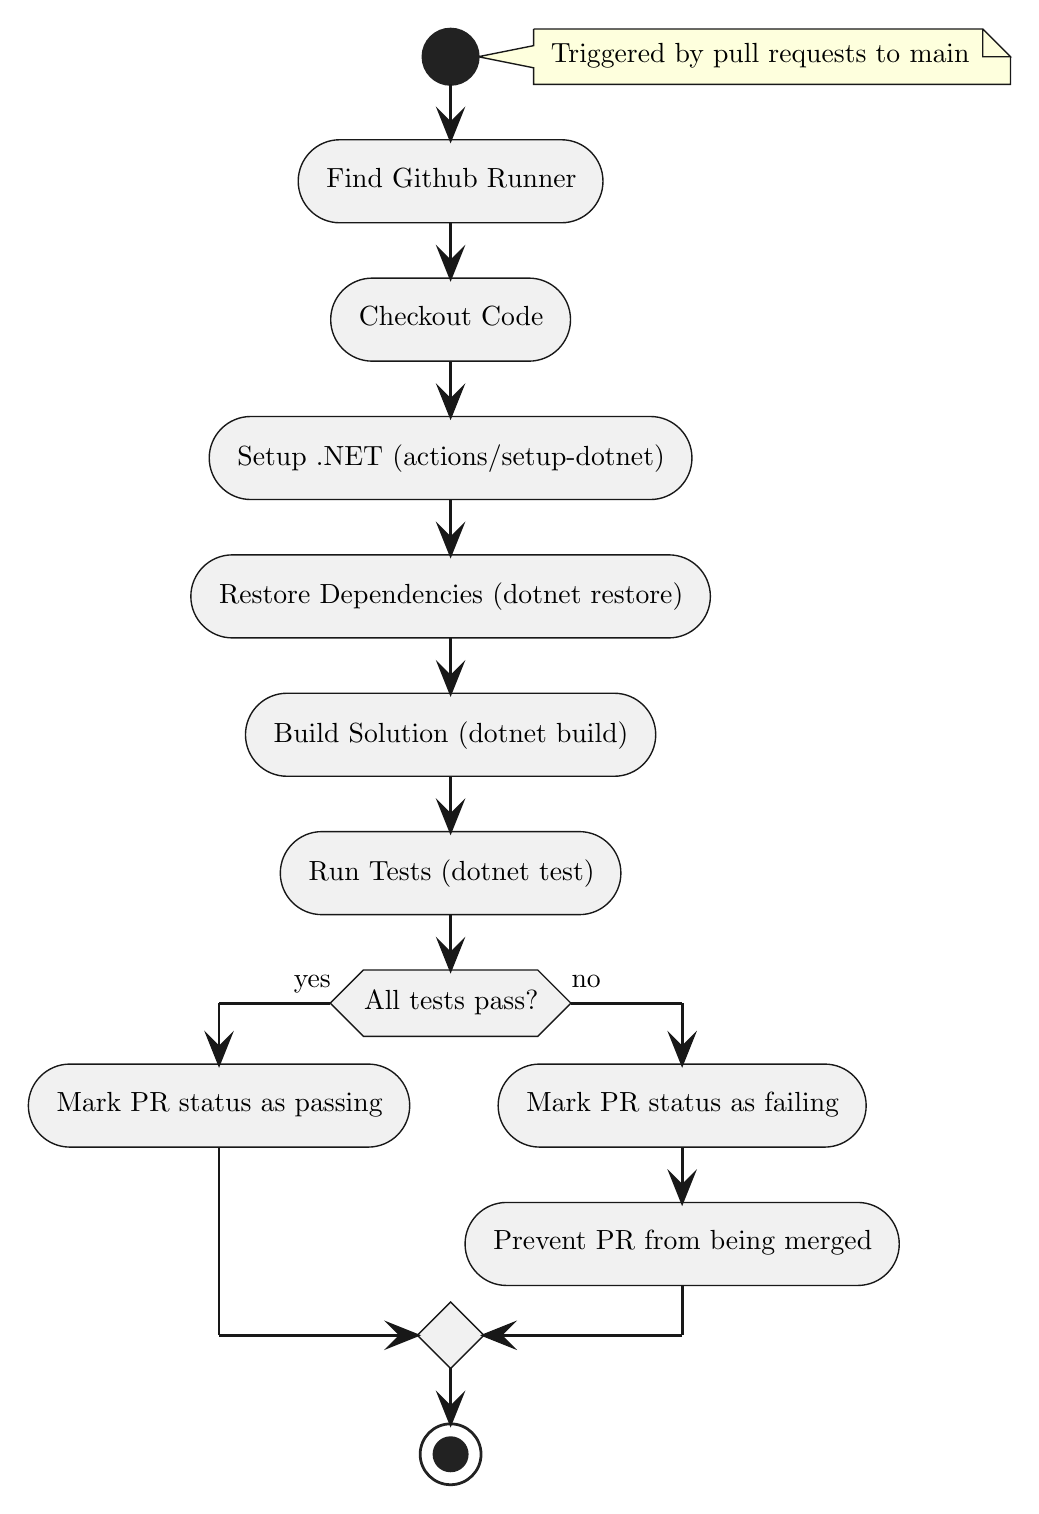
\begin{tikzpicture}[yscale=-1
,pstyle0/.style={color=plantucolor0001,fill=plantucolor0000,line width=0.5pt}
,pstyle1/.style={color=plantucolor0003,fill=plantucolor0003,line width=1.0pt}
,pstyle2/.style={color=plantucolor0001,fill=plantucolor0004,line width=0.5pt}
,pstyle4/.style={color=plantucolor0001,line width=1.0pt}
,pstyle5/.style={color=plantucolor0001,fill=plantucolor0001,line width=1.0pt}
]
\draw[pstyle0] (193.5725pt,10pt) -- (193.5725pt,16pt) -- (173.5725pt,20pt) -- (193.5725pt,24pt) -- (193.5725pt,30pt) -- (193.5725pt,30pt) -- (365.8825pt,30pt) -- (365.8825pt,30pt) -- (365.8825pt,20pt) -- (355.8825pt,10pt) -- (193.5725pt,10pt) -- (193.5725pt,10pt);
\draw[pstyle0] (355.8825pt,10pt) -- (355.8825pt,20pt) -- (365.8825pt,20pt) -- (355.8825pt,10pt);
\node at (199.5725pt,15pt)[below right,color=black,inner sep=0]{Triggered by pull requests to main};
\draw[pstyle1] (163.5725pt,20pt) ellipse (10pt and 10pt);
\draw[pstyle2] (108.5075pt,65pt) arc (180:270:15pt) -- (123.5075pt,50pt) -- (203.6375pt,50pt) arc (270:360:15pt) -- (218.6375pt,65pt) -- (218.6375pt,65pt) arc (0:90:15pt) -- (203.6375pt,80pt) -- (123.5075pt,80pt) arc (90:180:15pt) -- (108.5075pt,65pt) -- cycle;
\node at (118.5075pt,60pt)[below right,color=black,inner sep=0]{Find Github Runner};
\draw[pstyle2] (120.2425pt,115pt) arc (180:270:15pt) -- (135.2425pt,100pt) -- (191.9025pt,100pt) arc (270:360:15pt) -- (206.9025pt,115pt) -- (206.9025pt,115pt) arc (0:90:15pt) -- (191.9025pt,130pt) -- (135.2425pt,130pt) arc (90:180:15pt) -- (120.2425pt,115pt) -- cycle;
\node at (130.2425pt,110pt)[below right,color=black,inner sep=0]{Checkout Code};
\draw[pstyle2] (76.3575pt,165pt) arc (180:270:15pt) -- (91.3575pt,150pt) -- (235.7875pt,150pt) arc (270:360:15pt) -- (250.7875pt,165pt) -- (250.7875pt,165pt) arc (0:90:15pt) -- (235.7875pt,180pt) -- (91.3575pt,180pt) arc (90:180:15pt) -- (76.3575pt,165pt) -- cycle;
\node at (86.3575pt,160pt)[below right,color=black,inner sep=0]{Setup .NET (actions/setup-dotnet)};
\draw[pstyle2] (69.7075pt,215pt) arc (180:270:15pt) -- (84.7075pt,200pt) -- (242.4375pt,200pt) arc (270:360:15pt) -- (257.4375pt,215pt) -- (257.4375pt,215pt) arc (0:90:15pt) -- (242.4375pt,230pt) -- (84.7075pt,230pt) arc (90:180:15pt) -- (69.7075pt,215pt) -- cycle;
\node at (79.7075pt,210pt)[below right,color=black,inner sep=0]{Restore Dependencies (dotnet restore)};
\draw[pstyle2] (89.4525pt,265pt) arc (180:270:15pt) -- (104.4525pt,250pt) -- (222.6925pt,250pt) arc (270:360:15pt) -- (237.6925pt,265pt) -- (237.6925pt,265pt) arc (0:90:15pt) -- (222.6925pt,280pt) -- (104.4525pt,280pt) arc (90:180:15pt) -- (89.4525pt,265pt) -- cycle;
\node at (99.4525pt,260pt)[below right,color=black,inner sep=0]{Build Solution (dotnet build)};
\draw[pstyle2] (102.0375pt,315pt) arc (180:270:15pt) -- (117.0375pt,300pt) -- (210.1075pt,300pt) arc (270:360:15pt) -- (225.1075pt,315pt) -- (225.1075pt,315pt) arc (0:90:15pt) -- (210.1075pt,330pt) -- (117.0375pt,330pt) arc (90:180:15pt) -- (102.0375pt,315pt) -- cycle;
\node at (112.0375pt,310pt)[below right,color=black,inner sep=0]{Run Tests (dotnet test)};
\draw[pstyle2] (132.0825pt,350pt) -- (195.0625pt,350pt) -- (207.0625pt,362pt) -- (195.0625pt,374pt) -- (132.0825pt,374pt) -- (120.0825pt,362pt) -- (132.0825pt,350pt) -- cycle;
\node at (132.0825pt,357pt)[below right,color=black,inner sep=0]{All tests pass?};
\node at (106.7025pt,352pt)[below right,color=black,inner sep=0]{yes};
\node at (207.0625pt,352pt)[below right,color=black,inner sep=0]{no};
\draw[pstyle2] (11pt,399pt) arc (180:270:15pt) -- (26pt,384pt) -- (133.8pt,384pt) arc (270:360:15pt) -- (148.8pt,399pt) -- (148.8pt,399pt) arc (0:90:15pt) -- (133.8pt,414pt) -- (26pt,414pt) arc (90:180:15pt) -- (11pt,399pt) -- cycle;
\node at (21pt,394pt)[below right,color=black,inner sep=0]{Mark PR status as passing};
\draw[pstyle2] (180.755pt,399pt) arc (180:270:15pt) -- (195.755pt,384pt) -- (298.735pt,384pt) arc (270:360:15pt) -- (313.735pt,399pt) -- (313.735pt,399pt) arc (0:90:15pt) -- (298.735pt,414pt) -- (195.755pt,414pt) arc (90:180:15pt) -- (180.755pt,399pt) -- cycle;
\node at (190.755pt,394pt)[below right,color=black,inner sep=0]{Mark PR status as failing};
\draw[pstyle2] (168.8pt,449pt) arc (180:270:15pt) -- (183.8pt,434pt) -- (310.69pt,434pt) arc (270:360:15pt) -- (325.69pt,449pt) -- (325.69pt,449pt) arc (0:90:15pt) -- (310.69pt,464pt) -- (183.8pt,464pt) arc (90:180:15pt) -- (168.8pt,449pt) -- cycle;
\node at (178.8pt,444pt)[below right,color=black,inner sep=0]{Prevent PR from being merged};
\draw[pstyle2] (163.5725pt,470pt) -- (175.5725pt,482pt) -- (163.5725pt,494pt) -- (151.5725pt,482pt) -- (163.5725pt,470pt) -- cycle;
\draw[color=plantucolor0003,line width=1.0pt] (163.5725pt,525pt) ellipse (11pt and 11pt);
\draw[pstyle1] (163.5725pt,525pt) ellipse (6pt and 6pt);
\draw[pstyle4] (163.5725pt,30pt) -- (163.5725pt,50pt);
\draw[pstyle5] (159.5725pt,40pt) -- (163.5725pt,50pt) -- (167.5725pt,40pt) -- (163.5725pt,44pt) -- cycle;
\draw[pstyle4] (163.5725pt,80pt) -- (163.5725pt,100pt);
\draw[pstyle5] (159.5725pt,90pt) -- (163.5725pt,100pt) -- (167.5725pt,90pt) -- (163.5725pt,94pt) -- cycle;
\draw[pstyle4] (163.5725pt,130pt) -- (163.5725pt,150pt);
\draw[pstyle5] (159.5725pt,140pt) -- (163.5725pt,150pt) -- (167.5725pt,140pt) -- (163.5725pt,144pt) -- cycle;
\draw[pstyle4] (163.5725pt,180pt) -- (163.5725pt,200pt);
\draw[pstyle5] (159.5725pt,190pt) -- (163.5725pt,200pt) -- (167.5725pt,190pt) -- (163.5725pt,194pt) -- cycle;
\draw[pstyle4] (163.5725pt,230pt) -- (163.5725pt,250pt);
\draw[pstyle5] (159.5725pt,240pt) -- (163.5725pt,250pt) -- (167.5725pt,240pt) -- (163.5725pt,244pt) -- cycle;
\draw[pstyle4] (163.5725pt,280pt) -- (163.5725pt,300pt);
\draw[pstyle5] (159.5725pt,290pt) -- (163.5725pt,300pt) -- (167.5725pt,290pt) -- (163.5725pt,294pt) -- cycle;
\draw[pstyle4] (247.245pt,414pt) -- (247.245pt,434pt);
\draw[pstyle5] (243.245pt,424pt) -- (247.245pt,434pt) -- (251.245pt,424pt) -- (247.245pt,428pt) -- cycle;
\draw[pstyle4] (120.0825pt,362pt) -- (79.9pt,362pt);
\draw[pstyle4] (79.9pt,362pt) -- (79.9pt,384pt);
\draw[pstyle5] (75.9pt,374pt) -- (79.9pt,384pt) -- (83.9pt,374pt) -- (79.9pt,378pt) -- cycle;
\draw[pstyle4] (207.0625pt,362pt) -- (247.245pt,362pt);
\draw[pstyle4] (247.245pt,362pt) -- (247.245pt,384pt);
\draw[pstyle5] (243.245pt,374pt) -- (247.245pt,384pt) -- (251.245pt,374pt) -- (247.245pt,378pt) -- cycle;
\draw[pstyle4] (79.9pt,414pt) -- (79.9pt,482pt);
\draw[pstyle4] (79.9pt,482pt) -- (151.5725pt,482pt);
\draw[pstyle5] (141.5725pt,478pt) -- (151.5725pt,482pt) -- (141.5725pt,486pt) -- (145.5725pt,482pt) -- cycle;
\draw[pstyle4] (247.245pt,464pt) -- (247.245pt,482pt);
\draw[pstyle4] (247.245pt,482pt) -- (175.5725pt,482pt);
\draw[pstyle5] (185.5725pt,478pt) -- (175.5725pt,482pt) -- (185.5725pt,486pt) -- (181.5725pt,482pt) -- cycle;
\draw[pstyle4] (163.5725pt,330pt) -- (163.5725pt,350pt);
\draw[pstyle5] (159.5725pt,340pt) -- (163.5725pt,350pt) -- (167.5725pt,340pt) -- (163.5725pt,344pt) -- cycle;
\draw[pstyle4] (163.5725pt,494pt) -- (163.5725pt,514pt);
\draw[pstyle5] (159.5725pt,504pt) -- (163.5725pt,514pt) -- (167.5725pt,504pt) -- (163.5725pt,508pt) -- cycle;
\end{tikzpicture}
